%!TEX root = ../dokumentation.tex

\subsection{Skalierung}
\label{sec:Skalierung}
Wie bereits in \autoref{sec:Client-Server} angesprochen, bietet Redis die Möglichkeit mehrere Server zu verwenden.
Diese Server sind mit Hilfe einer \textit{Master-Slave}-Architektur miteinander verbunden.

Der Master-Server verwaltet weiterhin die gesammte Datenbank und empfängt Schreibanfragen der Clients.
Wenn Änderungen in der Datenbank erfolgen, werden diese Änderungen an die Slave-Server weitergegeben.
Das bietet den Vorteil, dass im Falle eines Ausfalls des Master-Knotens die Daten zum Einen nicht verloren gehen und zum Anderen schnell wieder zur Verfügung stehen.
Außerdem können die Slave-Knoten auch für Leseanfragen, wodurch die Last bei hohen Zugriffszahlen auf mehrere Server verteilt werden kann \cite[141]{3}.

Sollte einer der Slave-Knoten vorrübergehend ausfallen, bzw. nicht erreichbar sein und deshalb keine Änderungen empfangen können, findet eine automatische Synchronisation statt, sobald der Slave-Knoten wieder erreichbar ist.
Der Server erkennt anhand der fehlenden Antwort des Slaves, dass dieser nicht erreichbar ist und speichert die Änderungen in einer Warteschlange, dem sogenannten \textit{Backlog-Buffer}. 
Dieser Backlog-Buffer hat eine feste Größe, die bei der Konfiguration des Servers festgelegt werden kann. 

Übersteigt die Größe der Änderungen während der Abwesenheit des Slaves die des Buffers, findet ein sogenannter \textit{Full-Resync} statt.
Das bedeutet, dass der Slave-Knoten mit einem aktuellen Snapshot der Daten aus dem Master neu initialisiert wird \cite{Redis-Docs-Replication}.
Andernfalls findet ein sogenannter \textit{Partial-Resync} statt. Dabei werden die Änderungen des Backlog-Buffers an den Slave-Knoten übertragen und dort ausgeführt \cite[146 - 153]{3}.

Die Größe des Backlog-Buffers sollte anhand des erwarteten Datenaufkommens festgelegt werden. 
Bei größeren Datenmengen sollte der Buffer größer gewählt werden, damit nicht schon bei kurzen Ausfallzeiten der Buffer überläuft und anschließend ein gesammter Snapshot übertragen werden muss.
Trotzdem sollte der Buffer nicht zu groß gewählt werden, da die Synchronisation mittels Full-Resync bei großen Datenmengen performanter sein kann, als die Übertragung der Änderungen mittels Partial-Resync.

Neben einer einfachen Kopie der Daten auf mehrere Server, kann man sogenannte Redis-Cluster aufsetzen. Dabei wird die Datenbank auf mehrere Server zu verteilt.
Dieses Art der Erweiterung wird auch als horizontale Skalierung bezeichnet \cite{Fasel2016}.
In Redis wird dafür das sogenannte \textit{Data-Sharding} verwendet \cite{Redis-Docs-Scaling}.

Grundlage des Verfahrens ist eine Hash-Funktion mit Insgesamt 16384 Slots, bzw. möglichen unterschiedlichen Ergebnissen.
In einem Cluster erhält jeder Server einen bestimmten Bereich an Slots, die er verwaltet \cite{Redis-Docs-Scaling}.
Bei drei Servern könnte es zum Beispiel so aussehen, dass Server 1 die Slots 0 bis 5500, Server 2 die Slots 5501 bis 11000 und Server 3 die Slots 11001 bis 16383 verwaltet.
Dieses Verfahren kann jedoch, vorallem bei geringen Anzahl an Schlüsseln, dazu führen, dass die Daten nicht gleichmäßig auf die Server verteilt werden. 

Wenn nun ein Client eine Schreib- oder Leseanfrage an einen beliebigen der Server des Clusters sendet, wird die Hash-Funktion auf den Key der Anfrage angewendet.
Der Server weiß, welcher der Server für den entsprechenden Slot zuständig ist und leitet die Client an den entsprechenden Server weiter \cite{Redis-Docs-Scaling}.

Damit Daten bei einem Ausfall eines Servers nicht verloren gehen, kann zusätzlich das zuvor erwähnte Replikationsverfahren verwendet werden.

\begin{wrapfigure}{r}{0.7\textwidth}
    \centering
    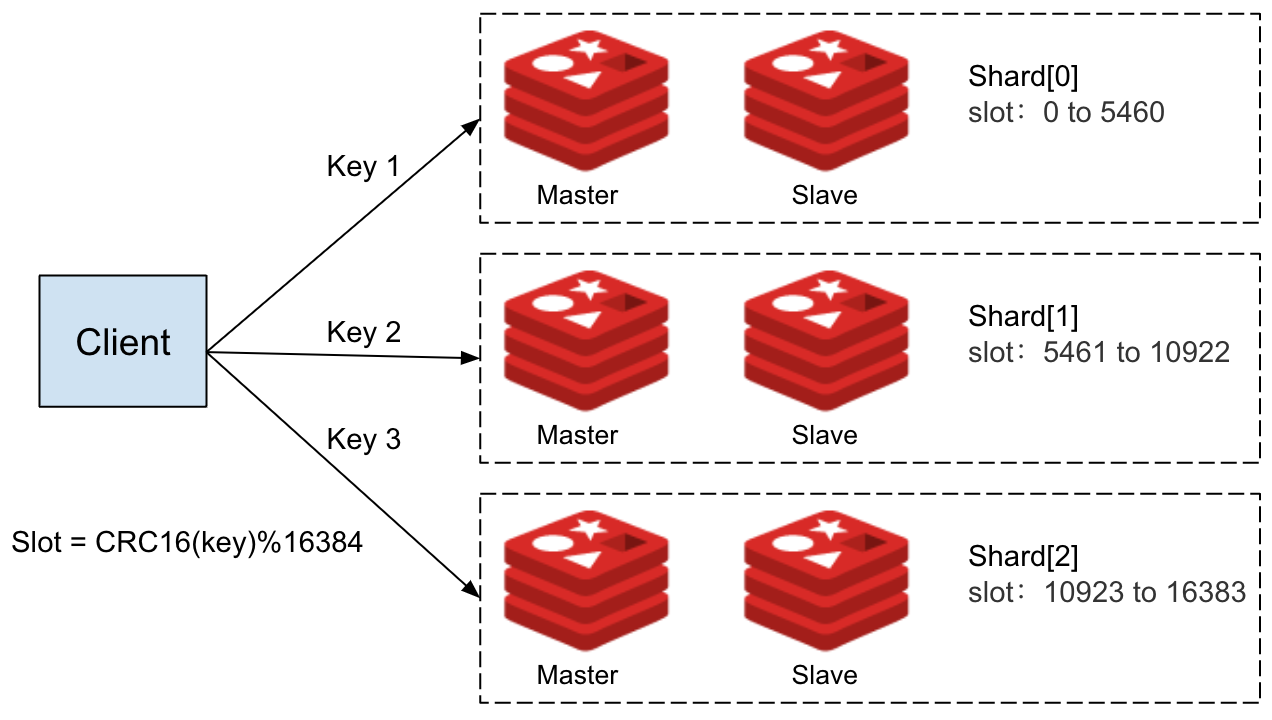
\includegraphics[width=0.7\textwidth]{images/redis-cluster.png}
    \caption{Redis-Cluster mit drei Master-Servern, \cite{aeraki}}
    \label{fig:redis-cluster} 
\end{wrapfigure}

Die \autoref{fig:redis-cluster} zeigt ein solches Beispiel.
Man sieht drei Master-Server. Jeder dieser Server ist für einen bestimmten Bereich an Slots zuständig.
In diesem Beispiel ist der Master des Shards 0 für die Slots 0 bis 5469, der Master des Shards 1 für die Slots 5470 bis 10922 und der Master des Shards 2 für die Slots 10923 bis 16383 zuständig.
Bei einer Anfrage wir der Slot berechnet und damit der zugehörige Server bestimmt. 

Um für eine Ausfallsicherheit zu sorgen, wurde in diesem Beispiel jeder Master-Server mit einem Slave-Server verbunden, der die Daten des Master-Servers repliziert und bei einem Ausfall einspringt.






